We next derive a formula for the sum of the angles
of the interior angles.
The proof provides intuition for other proofs we will encounter.
We have
\begin{theorem}\label{thm:triangle}
In the plane, the sum of the interior angles of a triangle is $\pi$.
\end{theorem}
\begin{proof}
Draw a line parallel to one edge through the opposite vertex.
By alternating interior angles in the plane, the sum of the angles
in the triangle equal a straight line.
See \figref{interior-angles} for an example. 
\end{proof}


 \begin{figure}[htb]
         \centering
        \begin{subfigure}[b]{0.35\textwidth}
         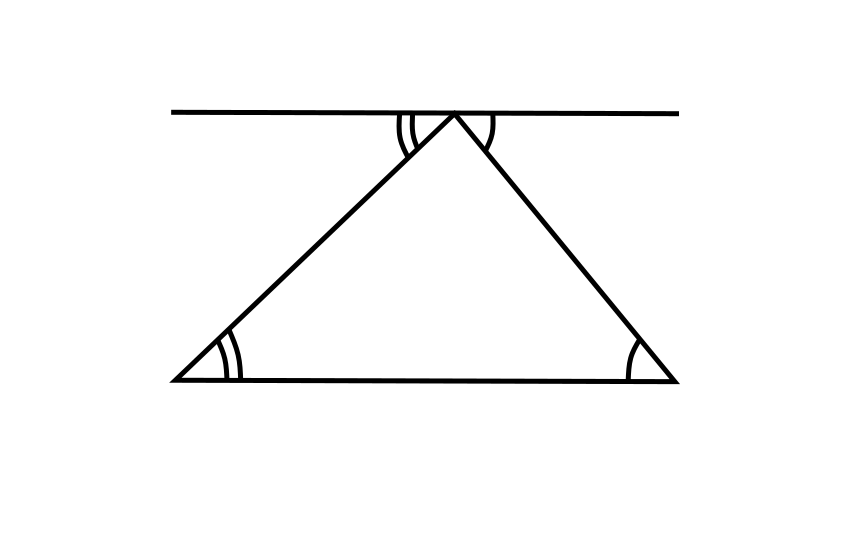
\includegraphics[width=\textwidth]{background/interior-triangle}
         \caption{Interior angles.}
 	 \label{fig:interior-angles}
       \end{subfigure}
         \hspace{1cm}
         \begin{subfigure}[b]{0.25\textwidth}
         \includegraphics[width=\textwidth]{background/exterior-angles-polygon}
         \caption{Exterior angles.}
          \label{fig:exterior-angles}
         \end{subfigure}
		\caption{(\subref{fig:interior-angles}) In the plane, the sum of the interior angles of a triangle is $\pi$.
 		 (\subref{fig:exterior-angles}) The sum of the exterior angles of a simple
		polygon is $2\pi$. Here
		$\alpha_1+\alpha_2+\alpha_3+\alpha_4+\alpha_5=2\pi$ note that $\alpha_4$ is negative.
 		\label{fig:simple-polygon}}
 \end{figure}

And we have
\begin{corollary}\label{cor:angles}
In the plane, any simple polygon $P$ with $n$ vertices,
the sum of the interior angles of $P$ is $(n-2)\pi$.
\end{corollary}

\begin{proof}
	Consider any simple polygon in the plane $P$ with $n$ vertices. 
	Then $P$ can be triangulated with $n-2$ triangles using only the vertices
	of $P$ \cite{orourke_computational_1994}.
	Thus, when we traverse $P$ we go around $n-2$ triangles each contributing
	$\pi$.
\end{proof}





\subsection{Triangulations}

Here we define simplicial complexes and triangulations.


\begin{definition}[Topological Space \cite{munkres}]
A \EMPH{topology} is a pair $(X,\tau)$, where $X$ is a set and
 $\tau$ is a collection of subsets $X$
satisfying:
	\begin{itemize}
		\item $\emptyset$ and $X$ are in $\tau.$
		\item the union of \emph{any} subcollection of elements in $\tau$ is  in $\tau.$
		\item the intersection of any \emph{finite} subcollection of elements in the $\tau$ is in $\tau.$
	\end{itemize}
A set $X$ with a specified topology $\tau$ is called a \EMPH{topological space}.
\end{definition}

We will work with a special type of topological spaces called manfiolds.

\begin{definition}[Manifold  \cite{tu2011}]
	A topological space $M$ is \EMPH{locally Euclidean of dimension $n$}
	if every point $p$ in $M$ has a neighborhood $U$ such that there is  a
	homeomorphism  $\phi$ from $U$ into and open  subset of $\R^n$.
	We call the pair $(U,\phi: U\to \R^n)$ a \EMPH{chart}, $U$ a \EMPH{coordinate neighborhood}
	and  $\phi$ a \EMPH{coordinate map}. 
A \EMPH{manifold} is a Hausdorff, second countable, locally Euclidean space.
\end{definition}

We will  consider two and three dimensional manifolds. Two dimensional
manifolds are called \emph{surfaces}.
The symbol $S$ in \eqnref{g-b} is a surface.
In order to perform computations on our manifolds, 
we often want a triangulation of our manifolds.
To define triangulations we need some preliminary definitions.



\begin{definition}[Independent Points]
Let $v_0,v_1,\ldots,v_k$ be points in $\R^n$. We call them \EMPH{affinely dependent}
if there are real numbers $\alpha_0,\alpha_1,\ldots,\alpha_k$, not all 0, such that
$\Sigma_{i=0}^k \alpha_iv_i=0$ and $\Sigma_{i=0}^k \alpha_i=0.$
Otherwise,  $v_0,v_1,\ldots,v_k$ are \EMPH{affinely independent}.

\end{definition}

\begin{definition}[Simplices]
A \EMPH{simplex} $\sigma$ is the convex hull of a finite affinely independent
set $A$ in $\R^n$. The points in  $A$ are  called vertices, the dimension
of  $\sigma$ is $|A|-1$.  The convex hull of a subset of vertices of a simplex
$\sigma$ is a \EMPH{face} of $\sigma$.
\end{definition}

\begin{definition}[Simplicial Complex]
A nonempty family $C$ of simplices is a \EMPH{simplicial complex} if the following
are satisfied:
\begin{itemize}
\item  Each face of any simplex is a simplex.
\item The intersection of $\sigma_1 \cap \sigma_2$ is a face of both $\sigma_1$ and 
$\sigma_2$.
\end{itemize}


\end{definition}

Some simplicial complexes are very similar to others.


\begin{definition}[Homeomorphism]
A  \EMPH{homeomorphism}  of topological spaces $(X_1,\tau_1$ and $(X_2,\tau_2)$
is a bijection $\phi:X_1\to X_2$ such that for every $\phi$ and $\phi^{-1}$ are continuous.
\end{definition}
For two topological spaces $X$ and $Y$ if there exists a  homeomorphism between
$X$ and $Y$ we say $X$ and $Y$ are topologically  equivalent and write  $X\cong Y.$

Manifolds can have a boundary denoted $\partial(M)$.
The dimension of $\partial(M)$ is one less than the dimension of $M$.
We are ready to define a triangulation.

\begin{definition}[Triangulation]
For a topological space $X$ and simplicial complex $C$ if $X\cong C$,
then $C$  is a \EMPH{triangulation} of $X$.
\end{definition}

 